\begin{frame}
\frametitle{Correlation is not causation - the importance of understanding what drives model prediction}
\begin{columns}
    \begin{column}{0.3\textwidth}
        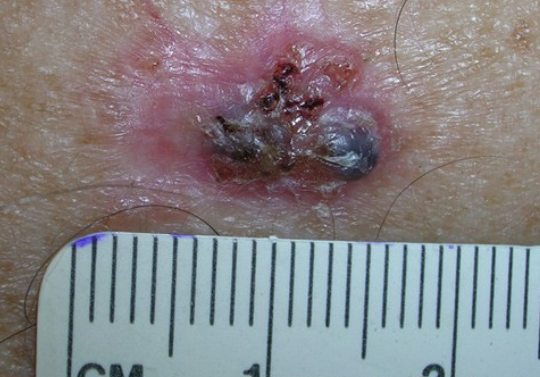
\includegraphics[width=1\textwidth]{./misc_images/skin_cancer.png}
    \end{column}
    \begin{column}{0.67\textwidth}
    \begin{itemize}
    \item In 2015 dermatologists Justin Ko and Robert Novoa used a Google image analysis network and trained it on 130,000 skin lesion images to recognise melanoma and other conditions. In a 2017 \emph{Nature} paper they reported that it out-performed 25 dermatologists.
        
    \item But a year they warned that the system was much more likely to classify any image with a ruler in it as cancerous; the model had learned that images with rulers in them were more likely to be cancerous.
    \end{itemize}
    \end{column}
\end{columns}
\end{frame}